\documentclass{../praktikum-ppt}

\author[Tew \& ...]{Teosofi Hidayah Agung}
\date{15 Maret 2025}
\title[Alpro 2 - Week 1]{Kebenaran Algoritma}
\institute[Matematika ITS]{Departemen Matematika\\ Institut Teknologi Sepuluh Nopember}


\begin{document}

{\usebackgroundtemplate{
  \tikz[overlay,remember picture] \node[opacity=0.2, at=(current page.center)]{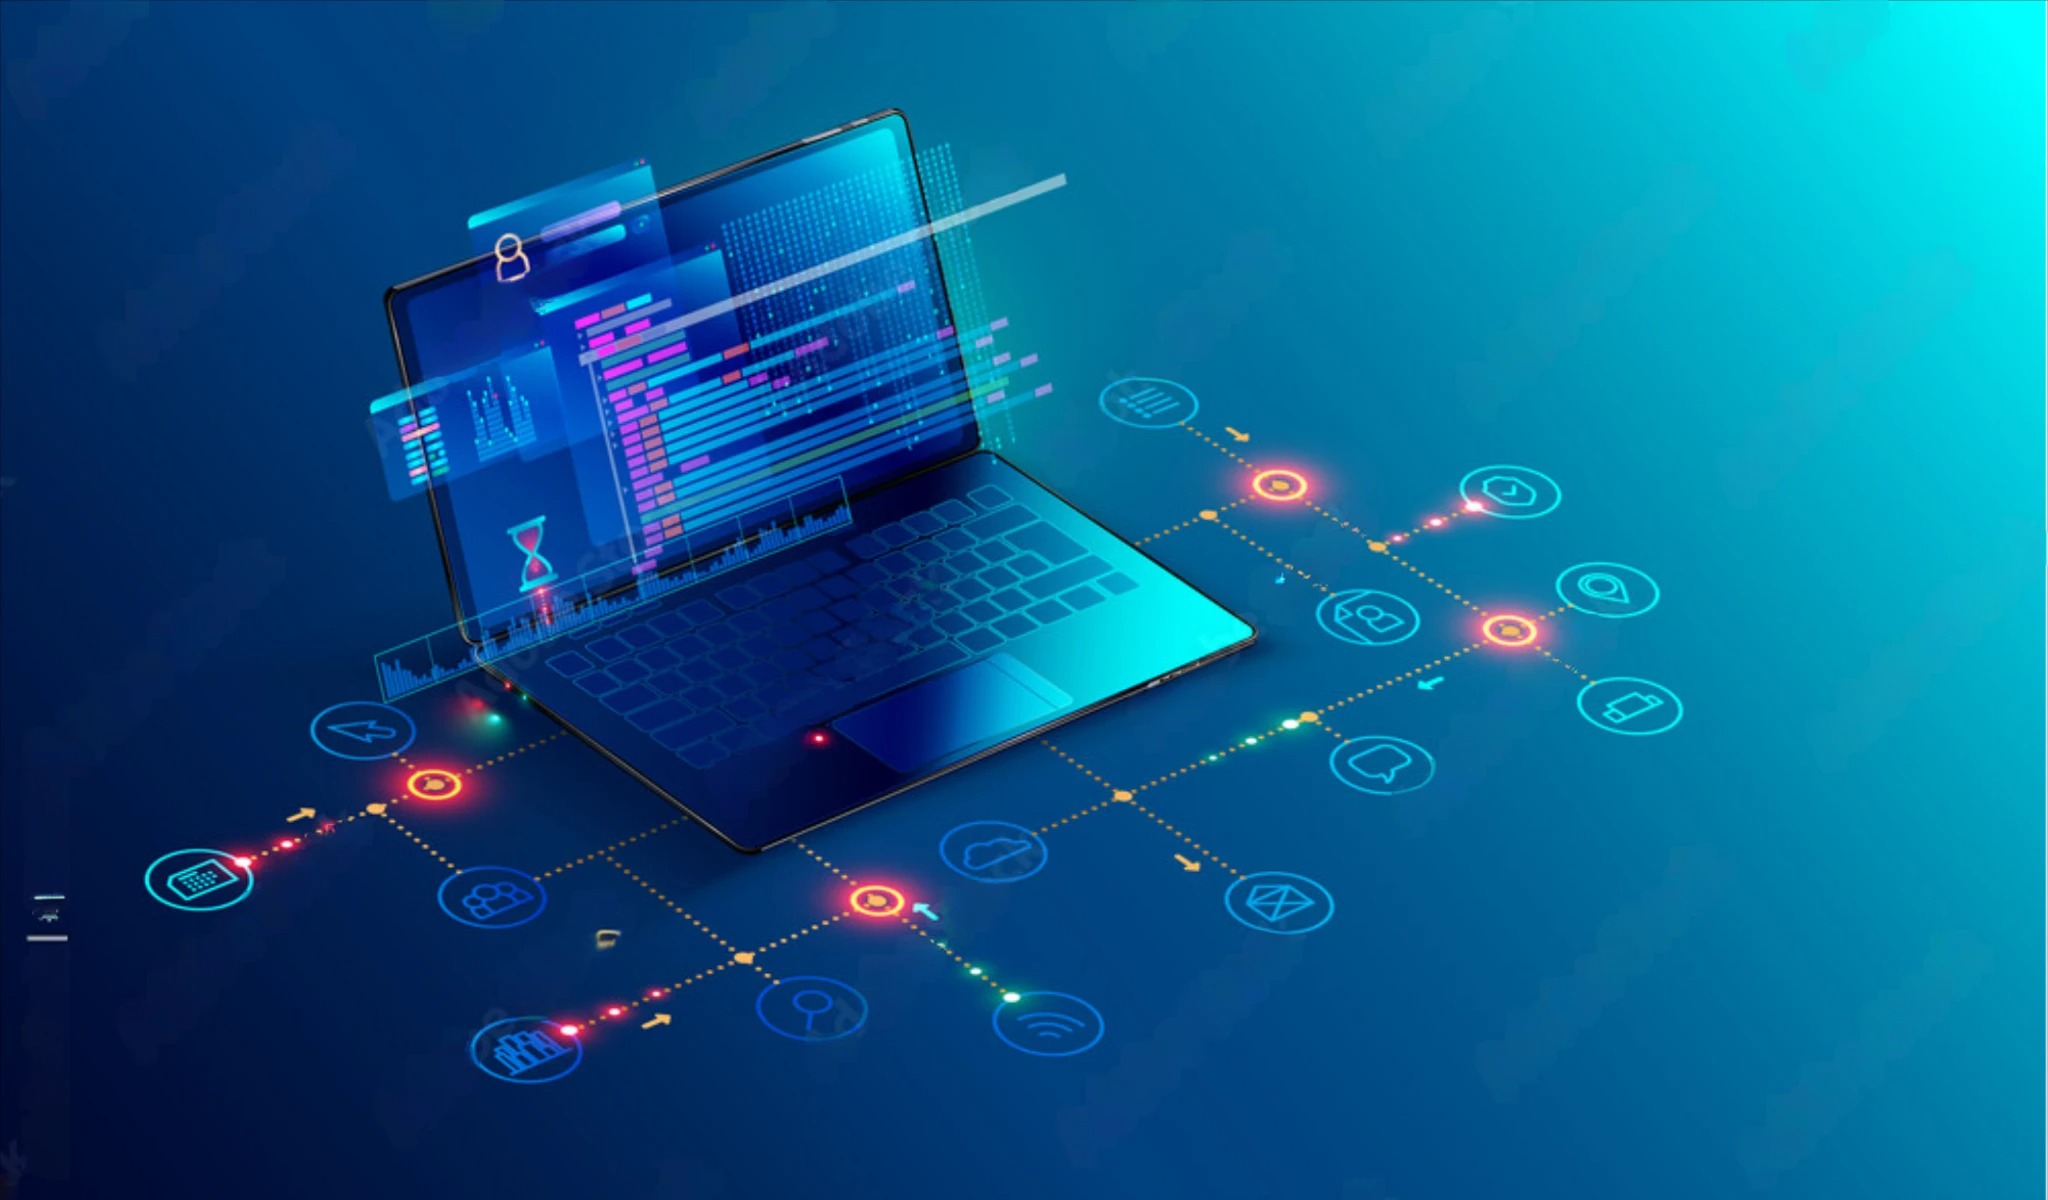
\includegraphics[width=\paperwidth]{bg_22}};}
\begin{frame}
  \titlepage
\end{frame}
}

\AtBeginSection{
    {\usebackgroundtemplate{
     \tikz[overlay,remember picture] \node[opacity=0.1, at=(current page.center)]{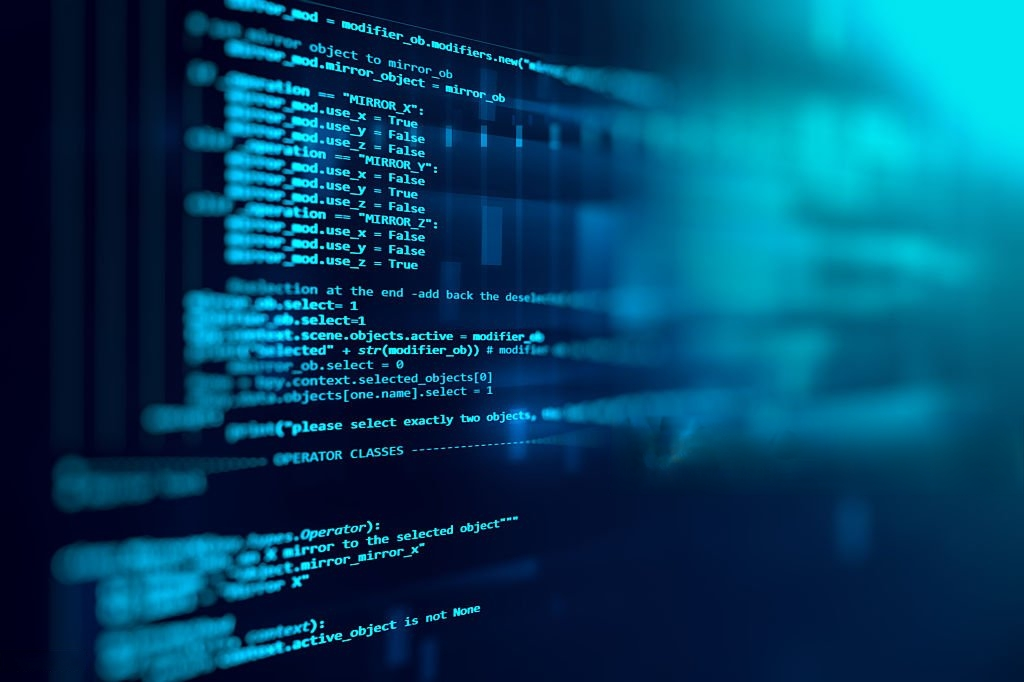
\includegraphics[width=\paperwidth]{code_bg}};}
    \begin{frame}{Daftar isi}
        \tableofcontents[currentsection]
        % \begin{tikzpicture}[overlay, remember picture] 
        %     \node at ([yshift=.5cm]current page.south east) [
        %         anchor = south east, 
        %         ] {
        %     \animategraphics[autoplay,loop,width=0.2\textwidth]{30}{Arisu Dance/Arisu Dance-}{0}{186}
        %     };
        % \end{tikzpicture}
    \end{frame}}
    }

    
    \begin{frame}
        \begin{masalah}
            Saat pertama kali melihat suatu kode program pastilah kita tidak akan langsung paham dengan apa yang dilakukan oleh kode tersebut. Sehingga diperlukan adanya \textbf{analisis} terhadap program apa yang dijalankan nantinya.\\

            Analisis dapat berupa apa saja, mulai dari analisa alur program, output yang dihasilkan, kompleksitas waktu dan ruang, dsb. Dalam materi kali ini kita cukup berfokus pada menganalisa kebenaran alur dan \textit{output} dari sebuah program.
        \end{masalah}
    \end{frame}

    \begin{frame}
      \begin{block}{Kebenaran Algoritma}
        \textit{\textbf{Correctness of Algorithm}} mengacu pada kepastian bahwa suatu algoritma memberikan hasil yang benar sesuai dengan spesifikasi masalah yang diberikan. Sebuah algoritma dikatakan benar (\textit{correct}), jika untuk setiap masukan yang valid, algoritma tersebut menghasilkan keluaran yang diharapkan dalam waktu yang wajar.
      \end{block}
      Analisa kebenaran algoritma cukup penting terlepas dari benar atau salah. Disisi lain analisa tersebut dapat membantu untuk menemukan sebuah solusi optimal dari suatu permasalahan.
    \end{frame}

    \section{Tipe-tipe Kebenaran}

    \begin{frame}
      \frametitle{\insertsection}
      \textit{Correctness} dalam algoritma biasanya dikategorikan menjadi dua bagian:
      \begin{enumerate}
        \item \textbf{Partial Correctness}
        \item \textbf{Total Correctness}
      \end{enumerate}
    \end{frame}

    \section{Teknik Pembuktian}
    \begin{frame}
      \frametitle{\insertsection}
    \end{frame}

    \section{Latihan}

\end{document}
